\documentclass[12pt,a4paper,oneside]{report}
\usepackage[utf8]{inputenc}
\usepackage[francais]{babel}
\usepackage{hyperref}
\usepackage{tabularx}
\usepackage[table]{xcolor}
\usepackage{pdfpages}
\title{Syllabus : Python et Raspberry Pi}
\author{Florence Blondiaux\and Jean-Martin Vlaeminck}
\date{06 août - 10 août 2018}

\usepackage{natbib}
\usepackage{graphicx}
\usepackage{listings}   
\usepackage{makecell}
\DeclareFixedFont{\ttb}{T1}{txtt}{bx}{n}{9} % for bold
\DeclareFixedFont{\ttm}{T1}{txtt}{m}{n}{9}  % for normal% incl. code langages info
\usepackage{color}
\definecolor{deepblue}{rgb}{0,0,0.5}
\definecolor{deepred}{rgb}{0.6,0,0}
\definecolor{deepgreen}{rgb}{0,0.5,0}
\newcommand\pythonstyle{\lstset{
  language=Python,
  backgroundcolor=\color{white}, %%%%%%%
  basicstyle=\ttm,
  otherkeywords={self},            
  keywordstyle=\ttb\color{deepblue},
  emph={MyClass,__init__},          
  emphstyle=\ttb\color{deepred},    
  stringstyle=\color{deepgreen},
  commentstyle=\color{red},  %%%%%%%%
  frame=tb,                         
  showstringspaces=False            
}}
\lstnewenvironment{python}[1][]
{
\pythonstyle
\lstset{#1}
}
{}
\usepackage{lipsum}                         % faux texte
\usepackage{fullpage}                       % utilisation de toute la page.
\usepackage{csvsimple}
\usepackage{multirow}
\usepackage{lscape}
\usepackage{xcolor}
\definecolor{darkgreen}{rgb}{0.13,0.54,0.13}
\usepackage{setspace}

\renewcommand{\familydefault}{\sfdefault}

\hyphenation{Python}
\hyphenation{PYTHON}






\begin{document}

\maketitle
\tableofcontents


\chapter{A quoi s'attendre?}

\vspace*{3cm}

Durant ce stage, nous allons aborder les points suivant :


\begin{minipage}[l]{0.70\textwidth}
	\begin{enumerate}
		\item Nous allons étudier le langage de programmation \textbf{PYTHON}. Ce langage va permettre aux étudiants d'interagir avec le raspberry pi et sera utile pour atteindre les objectifs fixés par le stage. Nous reprendrons les bases puis nous approfondirons la matière progressivement. De nombreux exercices accompagneront l'élève durant cet apprentissage.\\
		
		\item Nous découvrirons également comment interagir avec le \textbf{Raspberry Pi}. Nous verrons les bases de Linux, le c\oe{}ur du système d'exploitation du Raspberry Pi.
		
		% \item En fin de semaine nous réaliserons une petite \textit{station météo} ou un \textit{jeu video} sur le raspberry pi.
	\end{enumerate}
\end{minipage}
\hfill
\begin{minipage}[r]{0.30\textwidth}
	
\includegraphics[width=\textwidth]{Ressources/python.png}
	\bigskip
	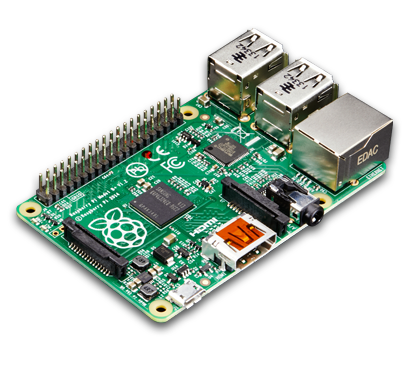
\includegraphics[width=\textwidth]{Ressources/pi.png}
\end{minipage}

\bigskip
Vous disposez chacun d'un Raspberry Pi permettant de résoudre les exercices proposés. Cependant n'hésitez pas à dialoguer avec vos voisins concernant votre solution. En informatique, nous appelons cette
technique le \textbf{pair programming}. Une telle méthode de travail
permet à la fois de rendre l'apprentissage plus agréable et plus
efficace.

\section*{Syllabus}
Ce syllabus 
%rédigé par Nicolas Houtain et Nathan Magrofuoco, a été modifié par Henri Devillez et Maxime Dimidschstein, étudiants en ingénieur civil à l'Université Catholique de Louvain. Cet ouvrage est partiellement inspiré du syllabus rédigé en 2012 par Gaëtan Biot et Sébastien De Fauw. 
est destiné à des élèves de 12 à 18 ans assistant aux stages d'été organisé par Technofutur TIC. Ce syllabus est un complément aux slides et aux discussions proposées durant les séances de ce stage. Il doit être complété par l'élève selon ses notes personnelles et les exercices réalisés durant la semaine.

Le syllabus a été écrit sous forme d'activités. Chaque activité peut être vue comme un exercice permettant de découvrir la matière. Cela permet d'apprendre la théorie de façon ludique et pratique.

\section{Plan de la semaine}

Ce plan est donné à titre informatif, il pourra être modifié selon les circonstances et les envies du groupe.\\
\begin{table}[h!]
	\begin{tabular}{|l|l|l|l|l|}
		\hline
		\rowcolor[HTML]{CA4242} 
		{\color[HTML]{000000} Lundi}                                                           & {\color[HTML]{000000} Mardi}                                       & {\color[HTML]{000000} Mercredi}                                           & {\color[HTML]{000000} Jeudi}                                   & {\color[HTML]{000000} Vendredi} \\ \hline
		\begin{tabular}[c]{@{}l@{}}Introduction au\\ Raspberry,\\ Premier \\programme\end{tabular} & \begin{tabular}[c]{@{}l@{}}Python\\ Types\\ Fonctions\end{tabular} & \begin{tabular}[c]{@{}l@{}}Python \\ Conditions\\ Boucles\end{tabular} & \begin{tabular}[c]{@{}l@{}}Coder un jeu\\ avec PyGame\end{tabular} & Radar avec le Raspberry %TODO                
		   \\ \hline
	\end{tabular}
\end{table}


%LE FAIRE SOUS TABLEAU COMME EN 2006 \\
%\begin{landscape}
%\begin{tabular}{|c|c|c|c|c|}
%\hline 
%Lundi & Mardi & Mercredi & Jeudi & Vendredi \\ 
%\hline 
%\multirow{2}{*}{} - Se présenter & - Révisions du lundi & - Révisions du mardi & - Révisions du mercredi & - Révisions du jeudi \\
% - Présentation de la semaine & - Présentation du projet & - Construire une classe & - Projet & - Projet \\
% - Questionnaire & & & & \\
%\hline 
%BREAK & BREAK & BREAK & BREAK & BREAK \\ 
%\hline 
%\multirow{2}{*}{} - Introduction à Java & - Première réflexion & - Projet & - Projet & - Projet \\
% - Exercices sur Java &  - Projet &  &  &  \\
%\hline 
%BREAK & BREAK & BREAK & BREAK & BREAK \\  
%\hline 
%\multirow{2}{*}{} - Classes, méthodes, .. & - Projet & - Projet & - Projet & - Projet \\
%- Exercices sur Java & - Première réflexion IA &  & - Améliorations IA &  \\
%\hline 
%BREAK & BREAK & BREAK & BREAK & BREAK \\ 
%\hline 
%\multirow{2}{*}{} - Bilan de la journée & - Révisions du lundi & - Révisions du mardi & - Révisions du mercredi & - Révisions du jeudi \\
% - Cloture & - Présentation du projet & - Construire une classe & - Projet & - Projet \\
%\hline 
%\end{tabular} 
%\end{landscape}







\chapter{Présentation de Python et installation des outils}

\section{Présentation de Python}
Python est un langage de programmation inventé par Guido van Rossum en 1990. Son nom est une référence à la série télévisée Monty Python, dont van Rossum était fan.

Au fil des années, le langage a évolué. En 2000, on voit apparaître \texttt{Python 2.0}, et en 2008, \texttt{Python 3.0}.
Actuellement, deux version de Python coexistent : \texttt{Python 2.7}, et \texttt{Python 3.6}. Nous utiliserons dans ce cours la dernière version.

Python est un langage très utilisé. Sa syntaxe simple en fait un des langages les plus appréciés pour écrire des \textit{scripts}. Il est aussi utilisé dans le monde scientifique, dans des domaines tels que la science des données et l'intelligence artificielle.

Dans ce cours, on utilisera le Python pour écrire des programmes, qu'on pourra exécuter sur un Raspberry Pi.

\section{Qu'est-ce qu'un programme?}
Les ordinateurs sont des outils très puissants, pour peu qu'on arrive à leur communiquer ce qu'on aimerait obtenir. On entend souvent dire qu'un ordinateur ne comprend qu'un langage très basique : le langage binaire, une suite de 0 et de 1. Du point de vue des microprocesseurs, on peut voir ça ainsi : soit le courant passe, soit il ne passe pas. En combinant ces deux états d'une manière bien précise, on peut effectuer des calculs.

Cependant, écrire un quelconque programme directement en binaire, c'est quasiment mission impossible, même pour un programme très basique. Il faut passer par une étape de traduction, et c'est ici que ça devient intéressant! L'idée générale est d'écrire du code dans un langage de programmation, et de le transformer en langage machine/binaire.

Il y a deux manières de traduire du code.
\begin{itemize}
    \item \emph{La compilation :} On convertit immédiatement le code en langage machine. L'avantage, c'est que l'ordinateur comprend directement. Par contre, il faudra recommencer cette étape pour chaque système d'exploitation différents (Windows, macOS, Linux, ...).
    \item \emph{L'interprétation :} on va ici passer par un intermédiaire : \textit{l'interpréteur}. C'est un programme qui lit et traduit le code en temps réel. C'est un processus plus lent, mais qui offre un grand avantage : on ne doit plus faire plusieurs versions pour chaque système d'exploitation, puisque c'est l'interpréteur qui se charge de la traduction! On dit d'un tel langage qu'il est \textit{multi-plateformes}.
\end{itemize}

%%% Au cours, on peut donner un exemple : compilation = traduire un texte en chinois et en arabe. Interprétation = le donner à un mec qui sait parler chinois et arabe. On doit pas traduire nous-même mais ça prend plus de temps.

Il existe une autre manière de classer les langages de programmation. Au plus ils ressemblent à du langage machine, au plus ils sont \textit{bas niveau}. Au contraire, au plus un langage de programmation se rapproche du langage humain, au plus il est \textit{haut-niveau}.

Le Python est un langage interprété, et haut-niveau, ce qui en fait un excellent choix pour débuter en programmation : on peut l'exécuter aisément sur de nombreux systèmes d'exploitation, et le code est assez lisible. Mais il ne faut pas s'y tromper : ce n'est pas parce qu'il est haut-niveau qu'il n'est pas puissant, bien au contraire!

\begin{figure}[t]
	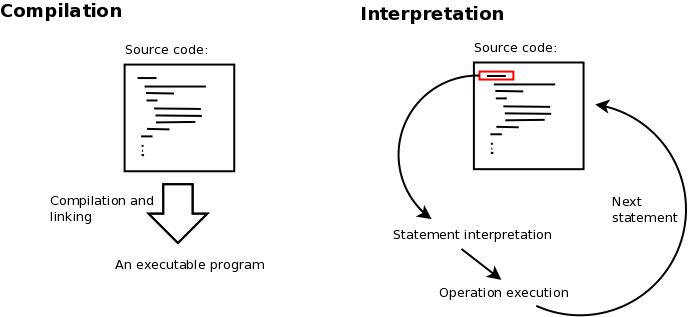
\includegraphics[width=\textwidth]{inter.png}
	\caption{Langage compilé vs langage interprété}
\end{figure}


\section{Environnement de développement}
Le Python est interprété, il nous faut donc un interpréteur! Il s'agit simplement d'un programme qui va lire notre code, et exécuter en temps réel les instructions qu'on lui donne.

Théoriquement, c'est le seul outil dont on a réellement besoin. Pratiquement, un développeur s'entoure d'une suite logicielle qui lui rend la vie bien plus facile. On utilisera énormément un \textit{éditeur de code}. C'est un éditeur de texte, à la manière de Microsoft Word, mais spécialisé dans un ou plusieurs langages de programmation. Il va notamment permettre de colorer le code pour le lire plus facilement, indenter automatiquement les lignes, les numéroter, etc.

Dans ce cours, nous allons utiliser l'éditeur de code (Atom) et l'interpréteur séparément.


\section{Premier programme}
Pour vérifier que l'installation s'est déroulée correctement et que vous disposez de tous les outils nécessaires, écrivons donc un premier programme!

Ouvrez votre éditeur de code, et créez un nouveau fichier. Dans l'éditeur copiez-collez le bout de code suivant :

\begin{python}
print("Tout fonctionne!")
\end{python}

Sauvegardez ce fichier et donnez-lui le nom \texttt{mon\_programme.py}. Ensuite, avec un terminal, déplacez vous dans le dossier où est stockée votre fichier. Une fois dans le dossier, executez la commande \texttt{python3 mon\_programme.py}. Si tout se passe correctement, une ligne de texte s'est affichée. Vous êtes maintenant prêts à démarrer l'apprentissage du Python!









\chapter{Programmer en Python}
%Ordre d'apprentissage à discuter
Maintenant que vous savez écrire un programme ainsi que l'exécuter et que vous avez écrit votre premier code, nous pouvons passer aux concepts de base de \textsc{Python}.

\section{Les bonnes pratiques du programmeur}
\begin{enumerate}
    \item Pas plus d'une instruction par ligne
    \item Aérer son code
    \item Faire \emph{très} attention à l'indentation du texte (surtout en python). 
    \item Commenter son code !
    \item Spécifier ses fonctions
\end{enumerate}
Ces 5 concepts ne vous parlent peut-être pas encore, mais vous seront familiers très bientôt. Ces règles permettent de différencier un bon programme d'un mauvais et ne s'arrêtent pas à \textsc{python} mais sont utilisées dans quasiment tous les langages de programmation. Nous vous encourageons donc vivement à vous en imprégner le plus rapidement possible.

\section{Affichage de texte}
L'instruction la plus simple est l'affichage de texte dans la console. Comme vous l'aurez deviné grâce à votre fonction test, l'affichage se fait grâce à l'instruction \texttt{print}.

\begin{python}
print("Le texte que je veux imprimer")
\end{python}

Il est préférable de ne pas mettre d'accents quand on imprime un texte dans la console, parce que toutes les configurations ne supportent pas leur affichage.

Pour effectuer un retour à la ligne, on peut terminer le texte par une suite de caractères spéciale : \lstinline{\n}.

Notez déjà qu'on peut imprimer autre chose que du texte brut : ce sont des variables, dont on parlera dans le chapitre suivant.
\subsubsection{Exercices}
    Modifier le code pour que l'ordinateur affiche "Bonjour maman"

\section{Commentaires}
Les commentaires sont des indications que le programmeur donne à quiconque voudrait lire son code. Les parties de texte commentées sont totalement ignorées par l'ordinateur lors de l'exécution d'un programme et, ainsi, n'affecte pas le code. En \textsc{Python}, on commente une phrase en la précédant du symbole \# et on commente un texte en le précédant de """ et en le terminant avec """ .
\begin{python}
print "Hello"
#Cette phrase est ignoree
print "World" #Cette phrase est ignoree
"""Toute
cette
phrase
est
ignoree"""
\end{python}

\section{Variables}
\label{variables}
\textbf{Qu'est ce qu'une variable ?} Les variables sont des symboles qui associent un nom à une valeur. La valeur est stockée dans la mémoire de l'ordinateur et le nom permet d'y accéder et/ou de modifier la valeur en tout temps. Une variable possède toujours un \textbf{type}. Ce dernier renseigne sur le "type" de la valeur stockée dans la variable. 

\begin{figure}[h!]
    \centering
    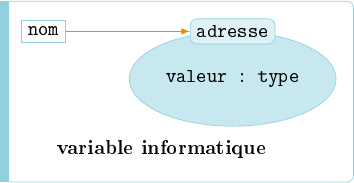
\includegraphics[width=7cm]{variable.png}
    \caption{Une variable}
    \label{variable}
\end{figure}

En \textsc{Python}, les noms de variables ne peuvent pas commencer par un chiffre, ni contenir d'espaces, ni contenir d'accents.

\begin{python}[caption = déclaration de variables]
nom_de_variable = valeur
#Exemples de variables correctes
variable1 = 1 #Une variable dont le nom est variable1 et la valeur est 1
b = "salut"
variable68452 = 0.50
variable_au_nom_tres_long = True
variable_lettre = 'a'
\end{python}


\subsection{Taille}

Les variables \textsc{Python} représentent une zone mémoire de l'ordinateur qui va stocker une certaine information. La taille d'une zone mémoire correspond à un ensemble de bits.

\begin{itemize}
    \item 1 \textit{bit} est le plus petit bout de donnée que l'on
    puisse stocker en mémoire. Il contient soit 1, soit 0.
    \item 1 octet (ou \textit{byte} en anglais) correspond à 8 bits
    \item 1 kilooctet (Ko) correspond à 1024 octets 
    \item 1 mégaoctet (Mo) correspond à 1024 Ko 
    \item 1 gigaoctet (Go) correspond à 1024 Mo 
\end{itemize}


\subsection{Type natif}\label{prim}

Python contient un ensemble de types natifs qui sont les types de données de \textbf{base}. Les types sont implicites lors de la déclaration d'une variable.

\begin{table}[!h]
    \centering
    \begin{tabular}{|c|c|}
        \hline
        Type & Description \\
        \hline
        \texttt{boolean} & Représente \textit{True} (vrai) ou \textit{False} (faux) \\
        \hline
        \texttt{str} & Représente une chaîne de caractères \\
        \hline
        %\texttt{byte} & & 1 octet \\
        %\texttt{short} & & 2 octets  \\
        \texttt{int} & Représente un entier\\
        %\texttt{long} & \multirow{-4}{*}{Représente un entier} & 8 octets \\
        \hline
        \texttt{float} & Représente un nombre à virgule\\
        %\texttt{double} & \multirow{-2}{*}{Représente un nombre à virgule} & 8 octets \\
        \hline
    \end{tabular}
    \caption{Type primitif}
    \label{table-primitifs}
\end{table}

\begin{python}[caption = Types de variables]
niveau = 'E'  #variable de type str
chaises = 12  #variable de type int
sonActif = False  #variable de type boolean
prixJeu = 12.50  #variable de type float
totalVoitures = 3453454  #variable de type int
\end{python}

Notons qu'on peut se renseigner sur le type d'une variable avec l'instruction \texttt{type(variable)}
\begin{python}[caption = Instruction type]
#Exemple
variable1 = 'a' 
variable2 = 2
variable3 = 12.50
print(type(variable1)) #Affiche "str"
print(type(variable2)) #Affiche "int"
print(type(variable3)) #Affiche "float"
\end{python}

\subsection{\textit{Cast} d'une variable}
Le mot \textit{cast} signifie qu'on impose un type à une variable. On impose un type à variable de la manière suivante :
\begin{python}[caption = Cast de variables]
nom_de_la_variable = type_que_je_veux(valeur)
#Exemples
a = int(1) # a est de type int
b = float(3) # b est de type float
c = float(4.5) # x est de type float
d = int(0.5) # Que se passe-t-il ?
\end{python}
%La raison qui pourrait nous pousser à faire ce choix est, par exemple, d'utiliser moins de mémoire pour représenter des variables qui en demandent moins. Si on s'en réfère au tableau \ref{prim}, on remarque qu'un \texttt{byte} consomme moins de mémoire qu'un \texttt{int} et que tous les deux permettent de représenter des entiers. On pourrait alors économiser de la mémoire en \textit{castant} nos variables en \texttt{byte} (\textsc{Python} représente les entiers par défaut en \texttt{int}).
Dans quels cas de figure est-ce utile de caster un nombre? Principalement parce qu'une opération s'effectue sur les mêmes types de données. On ne peut pas additionner "5" (la chaîne de caractères 5, un \texttt{str}!) avec 2 (un \texttt{int}!). Ici, on devrait donc d'abord caster le \texttt{str} en \texttt{int} avant l'opération. Mais il faut être prudent : que se passe-t-il si la chaîne de caractères ne peut être convertie en entier? Par exemple :
\begin{python}
int("salut") # Erreur!!!
\end{python}


\subsection{Affectation de variables}
Si vous avez bon souvenir, il était dit au tout début de la section \ref{variables} qu'on pouvait changer la valeur d'une variable. Pour ce faire, on égalise la variable à une nouvelle valeur. 
\begin{python}[caption = Réassignation de variables]
a = 2
print(a) #Affiche 2
a = 1
a = 4
print(a) #Affiche 4
a = "arbre" #Que se passe-t-il ?
print(a) #Affiche "arbre"
\end{python}

\subsection{Opérations arithmétiques}

On peut utiliser des opérateurs arithmétiques sur nos variables. Celles-ci vont être effectuées comme des opérations d'algèbre sur une calculatrice. Les opérations disponibles sont reprises dans le tableau ci-dessous
\begin{table}[!h]
    \centering
    \begin{tabular}{|c|c|}
        \hline
         Opération & Description\\
        \hline
        + & Addition \\
        \hline
        - & Soustraction \\
        \hline
        * & Multiplication \\
        \hline
        / & Division  \\
        \hline
        **  & Puissance \\
        \hline
        \% & Modulo \\
        \hline
    \end{tabular}
    \caption{Opérations arithmétiques}
    \label{oper}
\end{table}
\begin{python}
a = 4 + 6 #a vaut 10
a = ((a + a)/2)+1 #a vaut 11
b = a / 2 #b vaut 5
c = a**2 + b #c vaut 11^2 + 5 = 121 + 5 = 126
\end{python}


\subsection{Sucre syntaxique}

On dit souvent que les programmeurs sont des fainéants, et pour cause : ils cherchent à se faciliter la vie, et à réduire la taille des instructions qu'il tapent à longueur de journée! Ceux qui ont programmé les langages tel que \textsc{python} ont écrit des \textit{sucres syntaxiques} pour faciliter l'écriture et la lisibilité des programmes.

\begin{table}[!h]
    \centering
    \begin{tabular}{ccc}
        \texttt{x = x + 1} & $\Longleftrightarrow$ & \texttt{x += 1} \\
        \texttt{x = x + 1} & $\Longleftrightarrow$ & \texttt{x += 1} \\
        \texttt{x = x + 2} & $\Longleftrightarrow$ & \texttt{x += 2} \\
        \texttt{x = x - 2} &$\Longleftrightarrow$   & \texttt{x -= 2} \\
        \texttt{x = x / 2} &$\Longleftrightarrow$  & \texttt{x /= 2} \\
        \texttt{x = x * 2} &$\Longleftrightarrow$   & \texttt{x *= 2} \\

    \end{tabular}
    \caption{Quelques exemples de sucres syntaxiques}
\end{table}


\subsubsection{Exercices}

\begin{enumerate}
    \item Ecrivez un programme qui déclare les variables nécessaires pour effectuer le 
        calcul suivant :
        \begin{eqnarray*}
            x &=& 5\\
            y &=& x * 2\\
            w &=& ( y + x ) / 2\\
            y &=& y * x\\
        \end{eqnarray*}

    \item Quelles est la valeur des différentes variables après l'exécution de
        cette partie de code?

\begin{python}
x = 10
y = x * 2
w = y - 10
z = y / w
\end{python}
\end{enumerate}

\section{Le type \texttt{str}}
Maintenant que nous connaissons les types natifs, on peut aller un peu plus loin. Il y a quelque chose de très important à retenir : \textbf{En Python, tout est objet!} Mêmes les types de données natifs qu'on a vu précédemment sont des objets. Nous apprendrons plus tard à définir nos propres types de données, c'est-à-dire des \textbf{objets} qui ont été déclarés dans des \textbf{classes}. Dans cette section on va s'attarder sur un type de données qu'on a déjà rencontré : le \texttt{String} (ce qui veut dire \textit{chaîne} en anglais).

Un String est le type qui représente un texte. Tout texte entouré de guillemets est considéré comme un \texttt{String}.

\begin{python}[caption = type \texttt{String}]
#Exemples de Strings
v1 = "Ceci est une phrase"
v2 = ""
v3 = "3" #Est un String et non un int car il y a des guillemets!
v4 = "42.5"
v5 = "qpdjnqpuifnsfvsnvsdv5s1vd1s5v15xv4s5d"
print(type(v1)) #Imprime str (ce qui correspond a String)
\end{python}

\subsection{Opérations sur les \texttt{String}}
Chaque lettre du String est numérotée de par ordre croissant (commençant par zéro). Ainsi le String "Hello" possède la lettre \textit{H} en \texttt{0}, la lettre \textit{e} en \texttt{1}, etc... On accède à une lettre d'un \texttt{String} de la manière suivante :

\begin{python}[caption = Accès à String]
nom_du_string[numero_de_la_lettre] # Accede a la lettre d'un String
#Exemples
my_string = "Bonjour"
lettre_1 = my_string[0] #lettre_1 vaut 'B'
lettre_4 = my_string[3] #lettre_4 vaut 'j'
\end{python}

Attention à ne pas oublier que les numéros des lettres commencent à 0 et non à 1! C'est une faute très courante au début!

Des opérations courantes sur les \texttt{String} sont présentées dans le tableau ci-dessous.

Notez la syntaxe particulière des instructions lower et upper : le nom de la variable, suivi d'un point, suivi du nom de l'opération. Pour l'instant, utilisez-les telles quelles, on en reparlera dans le chapitre sur les classes et objets.

\begin{center}
\begin{tabularx}{\textwidth}{|>{\columncolor[gray]{0.9}} X|X|}
\hline
\rowcolor[gray]{0.8} \bf Opération & Description\\
\hline
\bf len(nom\_string) & Calcule la longueur d'un String \\
\hline
\bf nom\_string.lower() & Retourne le string en minuscule\\
\hline
\bf nom\_string.upper() & Retourne le string en majuscule\\
\hline
\bf str(nom\_variable) & Cast en String\\
\hline
\bf nom\_string1+nom\_string2 & Retourne les 2 String concaténées\\
\hline
\end{tabularx}
\end{center}

\subsection{Exercices}
\begin{enumerate}
\item \textbf{Exercice 1 :}    Concaténer les \texttt{Strings} "Hakuna Matata", "Mais quelle ", "phrase magnifique !" et affichez le résultat en majuscules ainsi que sa longueur.


\item \textbf{Exercice 2 :} Caster les Strings a = "2" et b = "125.2" en nombre pour calculer a/b.\footnote{a et b doivent être impérativement définis en String au départ !} 
\end{enumerate}

% \begin{table}[h!]
%     \centering
%     \begin{tabular}{|c|c|}
%         \hline
%          Opération & Description\\
%         \hline
%         len(nom\_string) & Calcule la longueur d'un String \\
%         \hline
%         nom\_string.lower() & Retourne le string en minuscule \\
%         \hline
%         nom\_string.upper() & Retourne le string en majuscule \\
%         \hline
%          str(nom\_variable) & Cast en String  \\
%         \hline
%         nom\_string1+nom\_string2  & Retourne les 2 String concaténés \\
%         \hline
%     \end{tabular}
%     \caption{Opérations String}
%     \label{operStr}
% \end{table}


\section{Interaction avec l'utilisateur}
Pour l'instant, nous nous limitons à des programmes dans lesquels toutes les valeurs sont définies avant l'exécution du programme. Ce qui nous limite assez fortement dans le genre de problèmes que l'on peut résoudre. Nous allons ici apprendre à demander à l'utilisateur de rentrer de l'information. 

On peut voir cette pratique comme lorsque Google vous demande un mot-clé à rechercher, lorsqu'un jeu vidéo vous demande un nom pour votre héros, etc...

La fonction qui permet cette opération s'appelle \texttt{input}. Par défaut, cette fonction convertit toutes les données entrées par l'utilisateur en \texttt{String} mais on peut imposer de recevoir un type en particulier en \textit{castant} la réponse de l'utilisateur dans le type désiré. 

\begin{python}[caption = fonction \texttt{input}]
answer = raw_input("ce_qu_on_affiche_a_l_utilisateur")
#Exemple
nom = input("Quel est votre nom ?")
prenom = input("Quel est votre prenom ?")
age = int(input("Quel est votre age ?"))
print "Bonjour " + nom + " " + prenom + " vous etes age de " + str(age) + " ans!"
\end{python}


\subsection{Exercice : } Faites un convertisseur qui demande à l'utilisateur des kilomètres et qui lui renvoie ce chiffre converti en miles en le remerciant d'avoir utilisé votre programme.

\textit{Aide : 1 km = 0.621 mile}
\label{convertisseur}

\section{Les conditions}
Nous effectuons chaque jour certaines actions plutôt que d'autres : "si je suis debout tôt, alors je vais chercher le petit déjeuner". En informatique, il est possible de faire raisonner une ordinateur d'une manière assez similaire\footnote{Pour les conditions hein, pas pour le petit déjeuner !}. % je suis mdr

Typiquement, les programmes informatiques utilisent des expressions dont on évalue la valeur selon certains opérateurs pour savoir si elle vaut \textbf{True} ou \textbf{False}.

L'action effectuée par l'ordinateur sera différente en fonction de la valeur (True ou False) de l'expression.

\subsection{Outils de comparaison}
Voici les opérations de comparaison disponibles en \textsc{Python} :

\begin{table}[!h]
    \centering
    \begin{tabular}{|c|c|}
        \hline
         Opération & Description\\
        \hline
        $==$ & Egalité \\
        \hline
        $!=$ & Différent \\
        \hline
        $>$ & Plus grand \\
        \hline
        $>=$ & Plus grand ou égal \\
        \hline
        $<$ & Plus petit  \\
        \hline
        $<=$  & Plus petit ou égal \\
        \hline
    \end{tabular}
    \caption{Comparaison}
    \label{operStr}
\end{table}

\begin{python}[caption = Quelques comparaisons en python]
a = 5 > 4 # a vaut True
b = 0.5 >= 1 # b vaut False
c = 1 > "salut" # Que se passe t il ?
\end{python}

\subsection{Opérateurs logiques}
Ce n'est pas tout ! On peut encore combiner ces expressions avec des opérateurs logiques.

Typiquement,on pourrait vouloir que deux conditions soient respectées, qu'au moins l’une des deux soit respectée ou qu'une condition ne soit pas respectée. Ceci est possible via les opérateurs \textsc{et}, \textsc{ou} et \textsc{non}. 
\paragraph{Table logique}
Chaque opérateur logique peut être défini par une table logique :

\begin{table}[!h]
    \begin{tabular}{cp{1cm}cp{1cm}c}
            \begin{tabular}{c|cc}
                \diaghead{\theadfont bbbbbbb}{a}{b}
                & \texttt{True} & \texttt{False} \\
                \hline
                \texttt{True} & \texttt{True} & \texttt{True} \\
                \texttt{False} & \texttt{True} & \texttt{False} \\
            \end{tabular}
            & &
            \begin{tabular}{c|cc}
                \diaghead{\theadfont bbbbbbb}{a}{b}
                & \texttt{True} & \texttt{False} \\
                \hline
                \texttt{True} & \texttt{True} & \texttt{False} \\
                \texttt{False} & \texttt{False} & \texttt{False} \\
            \end{tabular}
            & &
            \begin{tabular}{c|c}
                a & \\
                \hline
                \texttt{True} & \texttt{False} \\
                \texttt{False} & \texttt{True} \\
            \end{tabular}
            \\
            &&&& \\

            (a) OU & & (b) ET & & (c) NON \\
    \end{tabular}
    \caption{Table logique des opérateurs logiques}
\end{table}

\paragraph{En python}
En \textsc{python}, les opérateurs sont représentés à l'aide de
\texttt{and, or, not}.

\begin{table}[!h]
    \centering
    \begin{tabular}{|c|c|}
        \hline
        a OU b & a or b\\
        \hline
        a ET b & a and b \\
        \hline
        NON a & not a \\
        \hline
    \end{tabular}
    \caption{Opérateurs logiques en \textsc{Python}}
\end{table}

\subsubsection{Combinaisons}
Les opérateurs logiques ainsi expressions conditionnelles peuvent être combinés à l'infini pour former des expressions plus complexes. Cependant, comme pour les opérations mathématiques, il existe un ordre de priorité : d'abord \texttt{not}, puis \texttt{and}, puis \texttt{or}. Pour éviter les ambiguïtés et améliorer la lisibilité d'une expression complexe, on peut (et c'est conseillé!) y mettre des parenthèses.

\begin{python}[caption = Expressions booléennes]
a = True
b = False
c = a or b #c est vrai
d = a and b #d est faux
e = not b and a #e est vrai
f = (not (a and b)) or (not ((not d) and (a or e))) #f vaut True
\end{python}
\textbf{Exercices : } Evaluez les expressions suivantes :
\begin{python}[caption = Exercices d'expressions booléennes]
bool_one = False or not True and True
bool_two = False and not True or True
bool_three = True and not (False or False)
bool_four = not not True or False or not True
bool_five = False or not (True and True)
\end{python}
\subsubsection{Le \texttt{if}}
On peut représenter l'ensemble des exécutions possibles d'un programme comme un arbre de décision. Selon la valeur de certaines expressions, l'exécution du programme va prendre une direction ou
l'autre...


En résumé, certaines parties du code sont exécutées sous
certaines conditions!

\begin{figure}[!h]
    \centering
    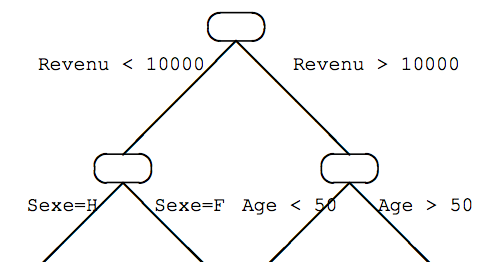
\includegraphics[width=7cm]{arbre.png}
    \caption{Arbre binaire de décision}
    \label{arbre}
\end{figure}

Afin de représenter ce choix, \textsc{Python} contient la clause \texttt{if} suivi d'une une expression booléenne et de \texttt{:}. Si la condition est vraie, le programme exécute toutes les instructions \textit{indentées}\footnote{Une expression indentée est une expression précédée d'une tabulation} qui suivent. Dans le cas contraire, ces instructions ne sont pas exécutées.

\begin{python}[caption = l'instruction if]
a = 10
if a > 5:
    print("Cette instruction est executee")
print("fin du code")
\end{python}
Il est aussi possible de donner un choix alternatif grâce à l'instruction \texttt{else:}. Si l'expression dans le \texttt{if} est \texttt{False}, le programme exécute alors le code \textit{indenté} qui suit le \texttt{else}.
\begin{python}
a = 10
if a < 5:
    print("Cette instruction n'est pas executee")
else:
    print("Cette instruction est executee")
print("fin du code")
\end{python}

\subsection{Le \texttt{elif}}
Vous pouvez construire des clauses \texttt{if} plus complexes en rajoutant des \texttt{elif}. Attention, à la première condition vraie rencontrée, on quitte la condition! Les expressions suivantes ne sont même pas évaluées.

\begin{python}[caption = utilisation de elif]
x = 200
if x > 10:
    print("A")
elif x > 100:
    print("B")
else:
    print("C")
# Seul 'A' est imprime, pas 'B' !!!
\end{python}
La clause \textbf{elif} permet d'augmenter l'embranchement 
(c'est-à-dire le nombre de choix possibles) de notre arbre de décisions!

\subsection{Code mort}

Lorsque vous utilisez des conditions, faites attention à ne pas créer du \textit{code mort}, c'est-à-dire du code qui ne sera jamais exécuté.
\begin{python}[caption = Exemple de code mort]
if False:
    print("Ce code n'est jamais execute!")
\end{python}

\subsubsection{Exercices}
    \begin{itemize}
	\item Définissez une variable \texttt{annee}, et imprimez "vrai" si l'année est bissextile. (\textbf{Aide :} une année est bissextile si elle est divisible par 4 et non divisible par 100, OU si elle est divisible par 400.)
	\item Ecrivez un code qui demande à l'utilisateur d'entrer un chiffre et imprime "Félicitations, votre chiffre est un multiple de 7" si le chiffre est divisible par 7. Et "Désolé, votre chiffre n'est pas un multiple de 7" sinon.
	\item \underline{Exercice récapitulatif}:     Affichez à l'écran "Timon ou Pumbaa?"\\
	Le but du programme est de vérifier que l'utilisateur écrit "Timon", et il n'a que deux essais.\\
	Si le deuxième essai est faux, on affiche "Tu prends la porte".\\
	Si l'utilisateur écrit Timon en un ou deux essais, on affiche "Bon choix!"\\
	Attention, vous ne pouvez utiliser que des conditions!\\
	Commentaires obligatoires!
\end{itemize}

\section{Boucles}
\subsection{La boucle \texttt{while}}

La boucle \texttt{while} est un outil très puissant en programmation. En français, cela correspond à dire \textit{tant que cette condition est vraie, j'exécute le code suivant}. En informatique, cela s'écrit avec le mot \texttt{while} suivi d'une expression booléenne et de \texttt{:}.
\subsubsection{Fonctionnement}
\begin{enumerate}
\item On évalue l'expression booléenne
\item Si l'expression est \textbf{False} : on ignore le code indenté qui suit le \textbf{while}.
\item Si l'expression est \textbf{True} : on exécute le code indenté qui suit \textbf{while} et retour à l'étape 1.
\end{enumerate} 
\begin{python}[caption = Exemple de boucle while]
"""Affiche tous les nombres de la table de 9 plus petits que 100"""
i = 0
while i <= 100:
	print("i vaut " + str(i))
	i = i+9	# Mise a jour de i
print("Fini")
\end{python}

\subsubsection{Attention à la boucle infinie!}

Comme vous avez pu le voir, la (ou les) variable de l'expression booléenne est mise à jour dans la boucle \texttt{while}. Dans le cas contraire, on ne sortira jamais de la boucle puisque la valeur de la condition de celle-ci ne sera jamais changée. Cet oubli de mise à jour crée ce qu'on appelle des boucles infinies et sont une erreur très courante. Ces dernières, en fonction de l'endroit où elle surgissent, peuvent faire planter votre programme.

\begin{python}[caption = Exemple de boucle infinie]
i = 0
while i < 10:
	print "Je suis dans la boucle"
print "Ce message ne s'affichera jamais"
\end{python}

\begin{figure}[!h]
    \centering
    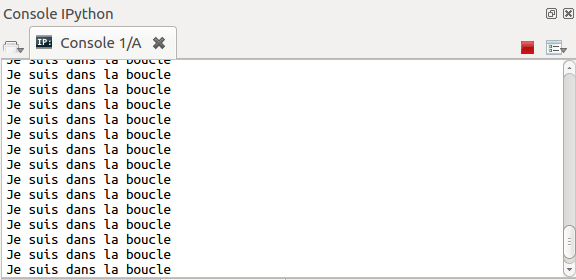
\includegraphics[width=7cm]{boucle_inf.png}
    \caption{Le programme ne s'arrête jamais}
    \label{arbre}
\end{figure}

\subsection{La boucle \texttt{for}}

La boucle \texttt{for} est, elle aussi, un réel passe-partout\footnote{Attention pas le même que celui de Fort-Boyard !} du programmeur. En \textsc{Python}, elle permet d'appliquer un code (\textit{indenté}) à chaque élément d'une structure de données\footnote{Par exemple un String ou une liste}. Elle commence toujours par le premier élément de la structure et finit par le dernier.

Pour ce faire, on écrit : \lstinline{for i in ma_structure}. Ici \texttt{i} (notez qu'on pourrait très bien choisir un autre nom de variable) est appelé \textit{itérateur}, c'est-à-dire que c'est lui qui prendra successivement la première valeur de la structure de données, puis la seconde, et ainsi de suite.

\begin{python}[caption = la boucle for]
"""Utilise une boucle for pour imprimer un string"""
s = "Hello World"
for i in s:
	print i
print "done" 
\end{python}

\subsection{Le \texttt{break}}
On peut, si on le désire, sortir à tout moment d'une boucle. Pour ce faire, on utilise le mot clé \textbf{break} à l'endroit où l'ont veut sortir. 

\begin{python}
i = 0
while(i<100):
	if i != 50:
		print i
		i = i+1
	else:
		break
\end{python}

\textbf{Attention : } un \texttt{break} est considéré comme une sortie "sale" d'une boucle. On ne l'utilise donc que lorsque cela est absolument nécessaire !

\subsection{Exercices : }
\begin{enumerate}
\item \textbf{Exercice 1 : } Améliorez votre convertisseur de l'exercice \ref{convertisseur} pour qu'il convertisse les unités de l'utilisateur jusqu'à ce que celui entre le mot "stop".  

\item \textbf{Exercice 2 : } Implémentez un programme qui prend un texte en entrée (fourni par l'utilisateur) et imprime chaque voyelle du texte. (Essayez avec un texte très long trouvé sur Internet...)

\item \textbf{Exercice 3 : } Implémentez un programme qui prend un texte en entrée (fourni par l'utilisateur) et qui imprime \textbf{True} si le texte contient un palindrome et \textbf{False} sinon. (\textbf{Aide :} un palindrome est un mot qui peut se lire dans les 2 sens. \textit{Exemple} : kayak, abcba, ...)
\end{enumerate}

\section{Listes}
Une liste est une structure de données permettant de regrouper des données de manière à pouvoir y accéder librement.

\begin{python}[caption = Exemples de listes]
jeuxVideos = ['HeartStone', 'LoL', 'WoW', 'ClubPenguin']
chiffres = [0, 1, 2, 3, 4, 5, 6, 7, 8, 9]
\end{python}

Accéder à un élément d'une liste se fait de la manière que pour un \texttt{String} (on commence à \textbf{0}).
En effet, un \texttt{String} est en réalité une liste de caractères!

\begin{python}[caption = Accès à une liste]
chiffres = [0, 1, 2, 3, 4, 5, 6, 7, 8, 9]

chiffre0 = chiffres[0]      #chiffre0 vaut 0
chiffre3 = chiffres[3]      #chiffre3 vaut 3
chiffres3a6 = chiffres[3:7] #chiffres3a6 vaut [3 4 5 6]
\end{python}

On peut modifier une liste de plusieurs façons : changer, supprimer, ajouter un ou plusieurs éléments.

\begin{python}[caption = Modification de liste]
my_list = ['a', 'b', 'c', 'd', 'e']

#Modification
my_list[3] = 'f'    #['a', 'b', 'c', 'f', 'e']
#Suppression
del my_list[3]      #['a', 'b', 'c', 'e']
my_list.remove('e') #['a', 'b', 'c']
#Ajout
my_list.append('d') #['a', 'b', 'c', 'd']
my_list + ['e']     #['a', 'b', 'c', 'd', 'e']
\end{python}

Les listes sont également assorties de quelques opérations très pratiques et souvent employées.

\begin{python}[caption = Opérations sur les listes]
my_list = ['a', 'b', 'c', 'd', 'e']

#Longueur de la liste
longueur = len(my_list)  #longueur vaut 5
#Presence d un element
'd' in my_list #vaut True 
'f' in my_list #vaut False
#Parcourir une liste
for x in my_list : print (x) #imprime abcde
#Retourner une liste
my_list.reverse() #my_list vaut ['e', 'd', 'c', 'b', 'a']
#Mettre une liste dans l ordre croissant
my_list.sort() #my_list vaut ['a', 'b', 'c', 'd', 'e']
\end{python}

\subsubsection{Exercices}
    \begin{enumerate}
	\item
		Créez une liste de Strings contenant au moins 5 fruits et légumes, puis triez la dans l'ordre alphabétique.
	\item
		Ajoutez à votre liste les éléments suivants \textbf{s'ils ne sont pas déjà présents} :
		['banane', 'tomate', 'rutabaga', 'reine-claude', 'patate']
\item
		Éliminez de votre liste tous les éléments dont la première lettre commence par la lettre \textbf{p}.
\end{enumerate}

\section{Fonctions}
Une fonction est un outil informatique qui encapsule une portion de code (une séquence d'instructions) et qui effectue une tâche bien spécifique (calcul, avertissement, affichage, ...).

L'utilisation d'une fonction se nomme \textit{appel d'une fonction}. Chaque appel de fonction contient des \textbf{arguments} qui sont les informations avec laquelle la fonction va travailler.

 Ce concept n'est pas nouveau, vous connaissez déjà plein de fonctions! Par exemple, la fonction \texttt{print()} qui prend en argument un \texttt{str} et l'imprime dans la console. \\
 
 Une fonction peut renvoyer une valeur, résultat de son exécution. Cette valeur s'appelle \textbf{la valeur de retour}. Autre exemple, la fonction \texttt{input} qui prend en argument un \texttt{str} (qui est la question posée à l'utilisateur) et retourne un \texttt{str} (qui est la réponse de l'utilisateur).\\
 
 \subsection{Créer ses propres fonctions}
 Utiliser des fonctions toutes faites c'est bien. En créer soi-même, c'est mieux ! 
 En \textsc{Python}, la création de fonction se fait par le code \texttt{def nom\_de\_la\_fonction(argument1, argument2, ...):}. Le code indenté qui suit cette instruction est le \textit{corps} de la fonction et correspond aux instructions que celle-ci exécutera à chaque appel. Pour renvoyer une valeur, on utilise le mot clé \texttt{return} suivi de la valeur qu'on souhaite renvoyer. Enfin, pour appeler une fonction, on utilise le nom de la fonction suivi des arguments qu'on veut lui passer entre parenthèses.
 
\begin{python}[caption = Exemple 1 : La fonction addition]
def addition(arg1, arg2): #Definition de la fonction addition
	return arg1+arg2
print(addition(3,4)) #Affiche 7
\end{python}
\begin{python}[caption = Exemple 2 : La fonction reverse]
def reverse(my_string): #Definition de la fonction qui inverse un String
	toReturn = ""
	for i in my_string:
		toReturn = i + toReturn
	return toReturn
print(reverse("esarhp eugnol zessa enU")) #Affiche Une assez longue phrase 
\end{python}

 \subsection{Exercices :}
 \begin{enumerate}
 \item Créez les fonctions \texttt{soustraction(arg1, arg2)}, \texttt{multiplication(arg1, arg2)}, \texttt{division(arg1, arg2)}, et \texttt{power5(arg)} qui, comme leurs noms l'indique font respectivement les opérations de soustraction, multiplication, division, mise à la puissance de 5. 
 \item Créez la fonction \lstinline{string_length(my_string)} qui affiche la longueur du texte en argument.
 %\item Implémentez le jeu du touché-coulé. (En cours)
 \end{enumerate}

\section{Portée des variables}
Les variables sont déclarées dans leur "bloc". Une variable déclarée dans une fonction est distincte des autres variables déclarées en dehors du corps de la fonction, et n'est plus accessible quand la fonction se termine. On appelle ce concept la \textbf{portée des variables}.

Dans l'exemple ci-dessous, on déclare deux variables appelées \texttt{x}, \textbf{mais ce ne sont pas les mêmes!} On s'en rend compte en exécutant le code : le \texttt{x} déclaré hors de la fonction n'est pas modifié après l'appel de la fonction.

\begin{python}
x = 10

def fonction():
    x = 20
    print(x)

fonction() # Imprime 20
print(x) # Imprime 10
\end{python}

On peut aussi utiliser utiliser le mot-clef \texttt{global} pour élargir la portée d'une variable, et la rendre globale. Ainsi, dans l'exemple suivant, quand Python rencontre le mot-clef \texttt{global} dans la fonction, il va regarder non seulement si \texttt{x} a été déclaré dans la fonction, mais aussi dans les "blocs" supérieurs. Dans ce cas, il trouve \texttt{x} déclaré à un niveau supérieur, et la fonction y a pleinement accès et peut la modifier.

\begin{python}
x = 10
print(x) # Imprime 10

def fonction():
    global x
    x += 10
    print(x)

fonction() # Imprime 20
fonction() # Imprime 30
print(x) # Imprime 30
\end{python}

Les variables globales paraissent pratiques : on la déclare une fois, et on peut l'utiliser partout. Cependant, dans un grand programme, elles deviennent bien vite une source de confusion, et ce n'est pas considéré comme une bonne pratique. On vous conseille donc de les utiliser avec modération.

\section{Modules}
On a déjà vu quelques fonctions inclues de base dans \textsc{Python}. Mais tout n'est pas présent, loin de là : un programme peut être utilisé pour afficher une interface graphique, travailler avec des images, accéder au web, faire des calculs mathématiques avancés, lire de l'audio ou de la vidéo, faire un jeu 3D... Ces quelques exemples montrent à quel point on peut se servir d'un seul langage pour faire à peu près tout et n'importe quoi!

Alors comment commencer? Chaque développeur pourrait bien sûr écrire de zéro chaque fonction donc il a besoin. Mais ce serait un travail immense, et on risque de faire des erreurs. Ainsi, les développeurs se sont organisés : ils ont regroupé des fonctions déjà écrites dans ce qu'on appelle des \textit{modules}. Il suffit d'importer un modules pour avoir accès à toutes ses fonctions!

Voici comment on importe un module, par exemple pour avoir accès à des fonctions mathématiques plus avancées :

\begin{python}
import math # importation du module math

x = math.ceil(8.728)
print(x) # imprime le premier entier superieur ou egal au parametre
\end{python}

Pour utiliser les fonctions du module, on écrit \lstinline{module.fonction()}.

Et si on n'a pas envie de taper à chaque fois le nom du module? On peut importer directement la fonction!

\begin{python}
from math import ceil # importe juste la fonction ceil

x = ceil(8.728)
print(x) # imprime le premier entier superieur ou egal au parametre
\end{python}

On peut aussi importer toutes les fonctions avec la ligne \lstinline{from module import *}.


% \section{(Optionnel) Dictionnaires}
% %TODO

% \section{(Optionnel) Tuples}
% %TODO

\section{Classes et objets}
Avant d’avancer plus en profondeur, il est utile de définir quelques mots de vocabulaire.
\begin{itemize}
    \item Une classe est une définition d’un concept. Elle peut être agrémentée d’attributs et de
fonctions pour la caractériser.
    \item Un objet est une instance d’une classe, c'est-à-dire que son comportement est défini par la
classe.
\end{itemize}

Si l’on prend l’exemple d’un véhicule, son plan de fabrication et de fonctionnement correspond à la classe.
Une voiture concrète, qui possède ses propres caractéristiques, correspond à un objet de cette classe. Et on peut construire plusieurs voitures à partir d'un seul plan, et les personnaliser en changeant ses options (attributs!).

Une classe possède des attributs qui sont eux-mêmes des objets (de différents types), et des méthodes qui sont des fonctions qui s'appliquent sur les objets de cette classe.
Le mot-clef \texttt{self} permet de référencer l'objet sur lequel on est en train de travailler.
Il est implicitement passé en argument à toutes les méthodes.
Le constructeur est une méthode particulière de la classe : il permet de créer un nouvel objet.

\begin{python}[caption = Exemple de classe]
class Vehicule:

    """Attributs"""
    
    #Valeurs par defaut
    nombreRoues = 4
    nombrePortes = 5
    nombrePlaces = 5
    couleur = 'noir'
    kilometres = 0
    
    """Methodes"""
    
    #Constructeur, permet de creer un objet vehicule avec un certain prix
    def __init__(self, prix):
        self.prix = prix
    
    #Modificateur, permet de changer la couleur
    def setColor(self, couleur):
        self.couleur = couleur
        
    #Calculateur de TVA (taxe de 21%)
    def tva(self):
        return self.prix * 0.21
    
    #Faire rouler le vehicule
    def rouler(self, distance)
        self.kilometres += distance
\end{python}

On peut ensuite utiliser cette classe pour créer une voiture, et s'en servir.

\begin{python}[caption = Exemple de classe]
voiture = Vehicule(10000)              #Cree une voiture au prix de 10 000 euros
facture = voiture.prix + voiture.tva() #Total a payer
voiture.rouler(200)                    #Roule sur 200km
voiture.setColor('red')                #Peint la voiture en rouge
voiture.rouler(150)                    #Roule sur 150km
print(voiture.distance)                #Affiche 350
\end{python}
%TODO

%\section{Héritage}
%TODO

%\section{Exercices supplémentaires}
%TODO










\chapter{Raspberry Pi}

\section{Présentation}
Le Raspberry Pi est un appareil étonnant : il tient dans la poche, coûte 35 euros, et il possède pourtant toutes les caractéristiques d'un vrai ordinateur : processeur, mémoire RAM, ports USB, port jack, port HDMI, port Ethernet... Les versions les plus récentes possèdent même des puces Wi-Fi et Bluetooth directement intégrées.

\begin{figure}[h!]
\begin{center}
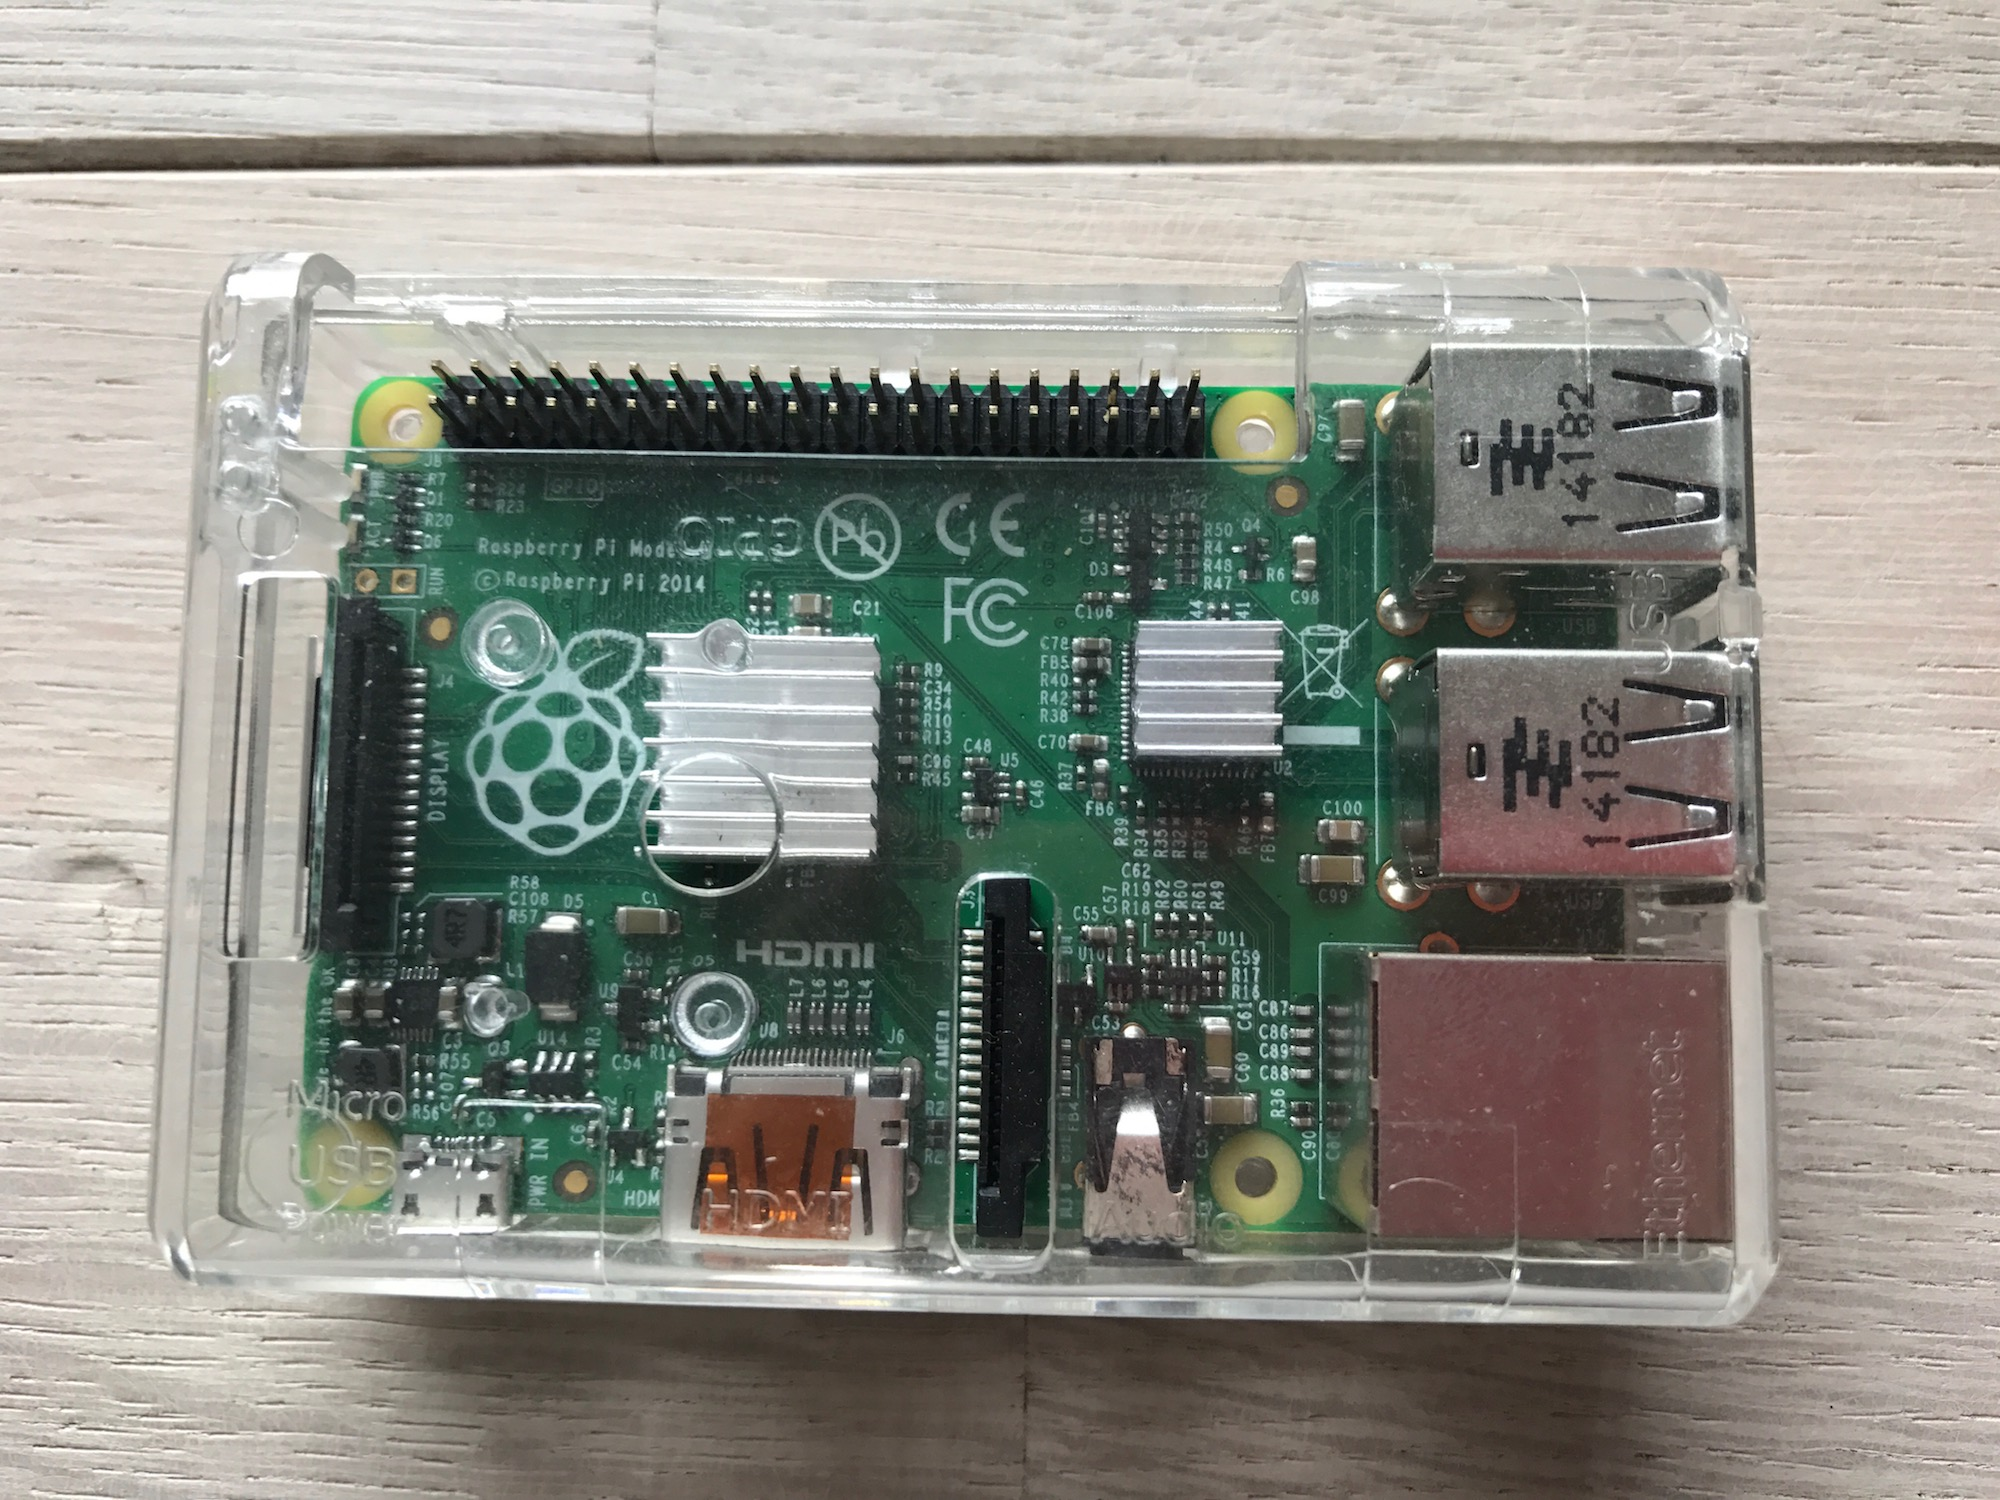
\includegraphics[width=10cm]{raspberry.JPG}
\end{center}
\caption{Raspberry Pi, première génération}
\label{raspberry}
\end{figure}

Il existe un connecteur très intéressant : les ports GPIO (\textit{General Purpose Input/Output} en anglais). Ils permettent d'envoyer ou de recevoir des signaux électriques, et de réagir en conséquence. On peut ainsi en faire de nombreux usages : allumer une LED, recevoir des informations d'un senseur, transformer une cafetière basique en une cafetière connectée... La seule limite est votre imagination!

Dans les sections suivantes, on va commencer par installer le système d'exploitation, puis on configurera l'appareil. On découvrira ensuite quelques utilisations d'un Raspberry Pi, dont certaines feront appel au Python!

\section{Mise en place}
Un Raspberry Pi n'a pas de disque dur intégré, ni d'autre système de stockage fixe. A la place, il utilise une simple carte micro-SD. Une faible capacité suffit : 8Go ou 16Go sont amplement suffisants pour commencer. On stockera dessus le \textbf{système d'exploitation}. Si on prévoit d'utiliser le Raspberry Pi pour traiter des gros fichiers, on peut bien sûr connecter un disque dur externe, ou un autre type de stockage, via les ports USB de l'appareil.

Mais même en ayant installé un système d'exploitation, on ne pourra pas faire grand chose de cette petite carte verte... Il nous manque des périphériques élémentaires : un écran, un clavier, et une souris!
On connecte le clavier et la souris via les ports USB. Quant à l'écran, le Raspberry Pi peut y être connecté avec son port HDMI.
En pratique cependant, on accède souvent au Raspberry Pi à distance via un autre ordinateur, ainsi on n'a pas besoin de connecter un clavier ou un écran. Nous apprendrons à faire cela dans un prochain chapitre.

Enfin, il n'y a pas de bouton ON/OFF sur le Raspberry Pi. Pour l'allumer, il suffit de le brancher à un prise électrique via son cordon d'alimentation.

\section{Installation de l'OS}
Installons donc le système d'exploitation. Il faut d'abord savoir qu'il n'y en a pas qu'un seul : le Raspberry Pi est pensé pour être un appareil multi-usages, il y a donc plusieurs systèmes d'exploitation! On peut y installer un système bureautique classique, semblable à Windows ou macOS, ou bien en faire une box multimédia qu'on connecte à la télévision. D'autres distributions sont dédiées à l'Internet des objets, c'est-à-dire les objets connectés.

Pour cette introduction, on va installer le système d'exploitation le plus connu, et le plus utilisé : Raspbian. Concrètement, il s'agit d'un système basé sur Linux, appelé Debian, mais optimisé pour fonctionner sur un Raspberry Pi.

Commencez par télécharger l'\textbf{image disque} de Raspbian sur \url{https://www.raspberrypi.org/downloads/raspbian/}. C'est un fichier assez lourd, il pèse en effet quelques gigaoctets.

Une fois l'image disque téléchargée, il faut la graver sur la carte micro-SD. Il y a plusieurs moyens d'y parvenir. Pour les plus téméraires, on peut utiliser la console; des instructions sont disponibles sur le site officiel\footnote{Voir en bas de cette page : \url{https://www.raspberrypi.org/documentation/installation/installing-images/README.md}}. Cependant, ce sont des manipulations avancées. On se contentera d'utiliser le programme Etcher, disponible sur Windows, macOS, et Linux en général, et très facile d'utilisation. Vous pouvez le télécharger ici : \url{https://etcher.io}.

\begin{figure}[h!]
\begin{center}
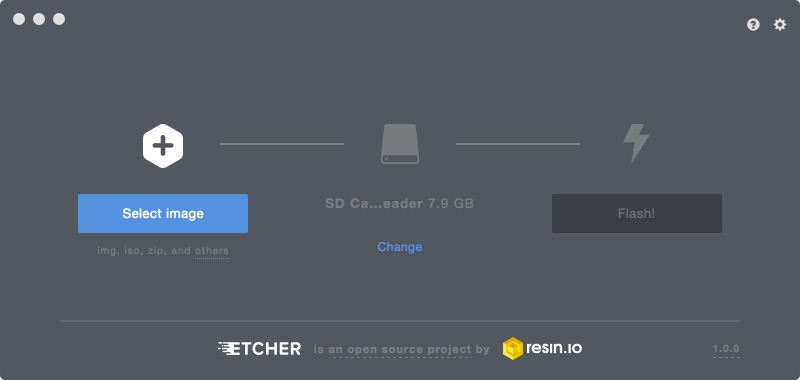
\includegraphics[width=10cm]{etcher.jpg}
\end{center}
\caption{L'interface très simple de Etcher}
\label{etcher}
\end{figure}

Sur la figure \ref{etcher}, on peut voir la seule et unique fenêtre de Etcher. En cliquant sur le bouton de gauche, vous pouvez sélectionner l'image disque. Elle devrait être au format \texttt{.img}. Si ce n'est pas le cas (\texttt{.zip} par exemple), il faudra la \textit{dézipper}. \textit{7zip} sur Windows et \textit{The Unarchiver} sur macOS permmettent de le faire.

Avec le bouton du milieu, sélectionner votre carte micro-SD dans l'explorateur de fichiers. Enfin, appuyez sur le bouton de droite "Flash!" pour graver l'image disque. L'opération prend environ 10 minutes.

Un fois ceci fait, profitez-en déjà pour activer une fonctionnalité dont nous aurons besoin : le SSH, qui permet d'accéder au Raspberry Pi à distance. Seulement, il y a quelques mois, une attaque informatique de grande envergure a utilisé des milliers d'appareils connectés pour affaiblir les serveurs des plus grands sites Internet. Suite à ça, l'entreprise qui produit les Raspberry Pi a décidé de désactiver le SSH par défaut, par mesure de sécurité.

Ce n'est pas grave, on peut le réactiver! Il suffit de créer n'importe quel fichier (avec un éditeur de texte par exemple), peu importe son contenu, de le nommer \texttt{ssh} (sans extension), et de l'ajouter à la \textbf{racine} de la carte micro-SD. La racine constitue le tout premier niveau d'un disque; c'est simplement la première chose qu'on voit quand on ouvre le disque dans un explorateur de fichiers.

Lors du premier démarrage, le Raspberry Pi détectera la présence du fichier, activera le SSH, et puis supprimera le fichier, tout simplement.

\section{Terminal}
Aujourd'hui, tous les ordinateurs grand public ont une interface graphique, qu'on pilote principalement avec la souris; le clavier ne sert plus qu'à taper du texte. Cependant, il n'en a pas toujours été ainsi! Au début de l'informatique, toutes les interactions se faisaient au clavier, dans ce qu'on appelle la \textbf{console}, ou \textbf{terminal} (figure \ref{terminal}).

\begin{figure}[h!]
\begin{center}
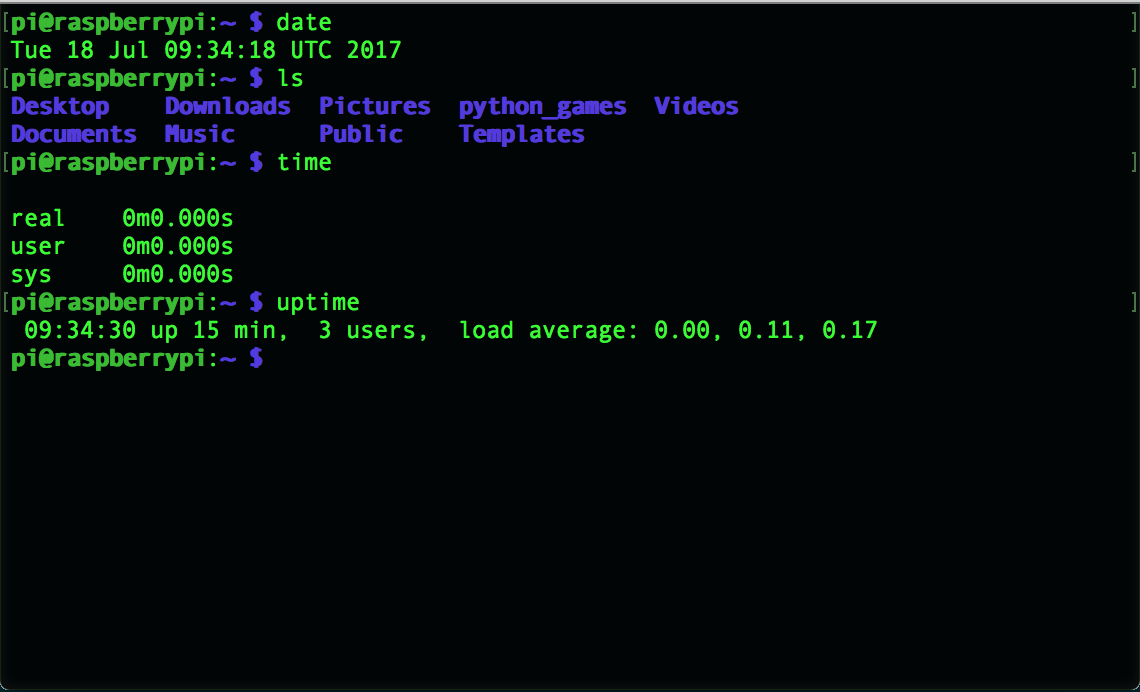
\includegraphics[width=10cm]{ssh.png}
\end{center}
\caption{Le terminal}
\label{terminal}
\end{figure}

Bien que sur Windows ou macOS, on n'utilise presque plus le terminal, il a encore une certaine utilité sur les distributions Linux, dont Raspbian fait partie.
Il existe des commandes très pratiques pour rapidement mettre à jour ses programmes, ou bien configurer certains aspects du Raspberry Pi.

On accède au terminal du Raspberry Pi en appuyant sur la quatrième icône de la barre des menus (voir figure \ref{interface}).

\section{Accéder au Raspberry Pi}
Il existe de nombreuses manières d'accéder au Raspberry Pi. Nous détaillerons ici les principales.

\begin{figure}[h!]
\begin{center}
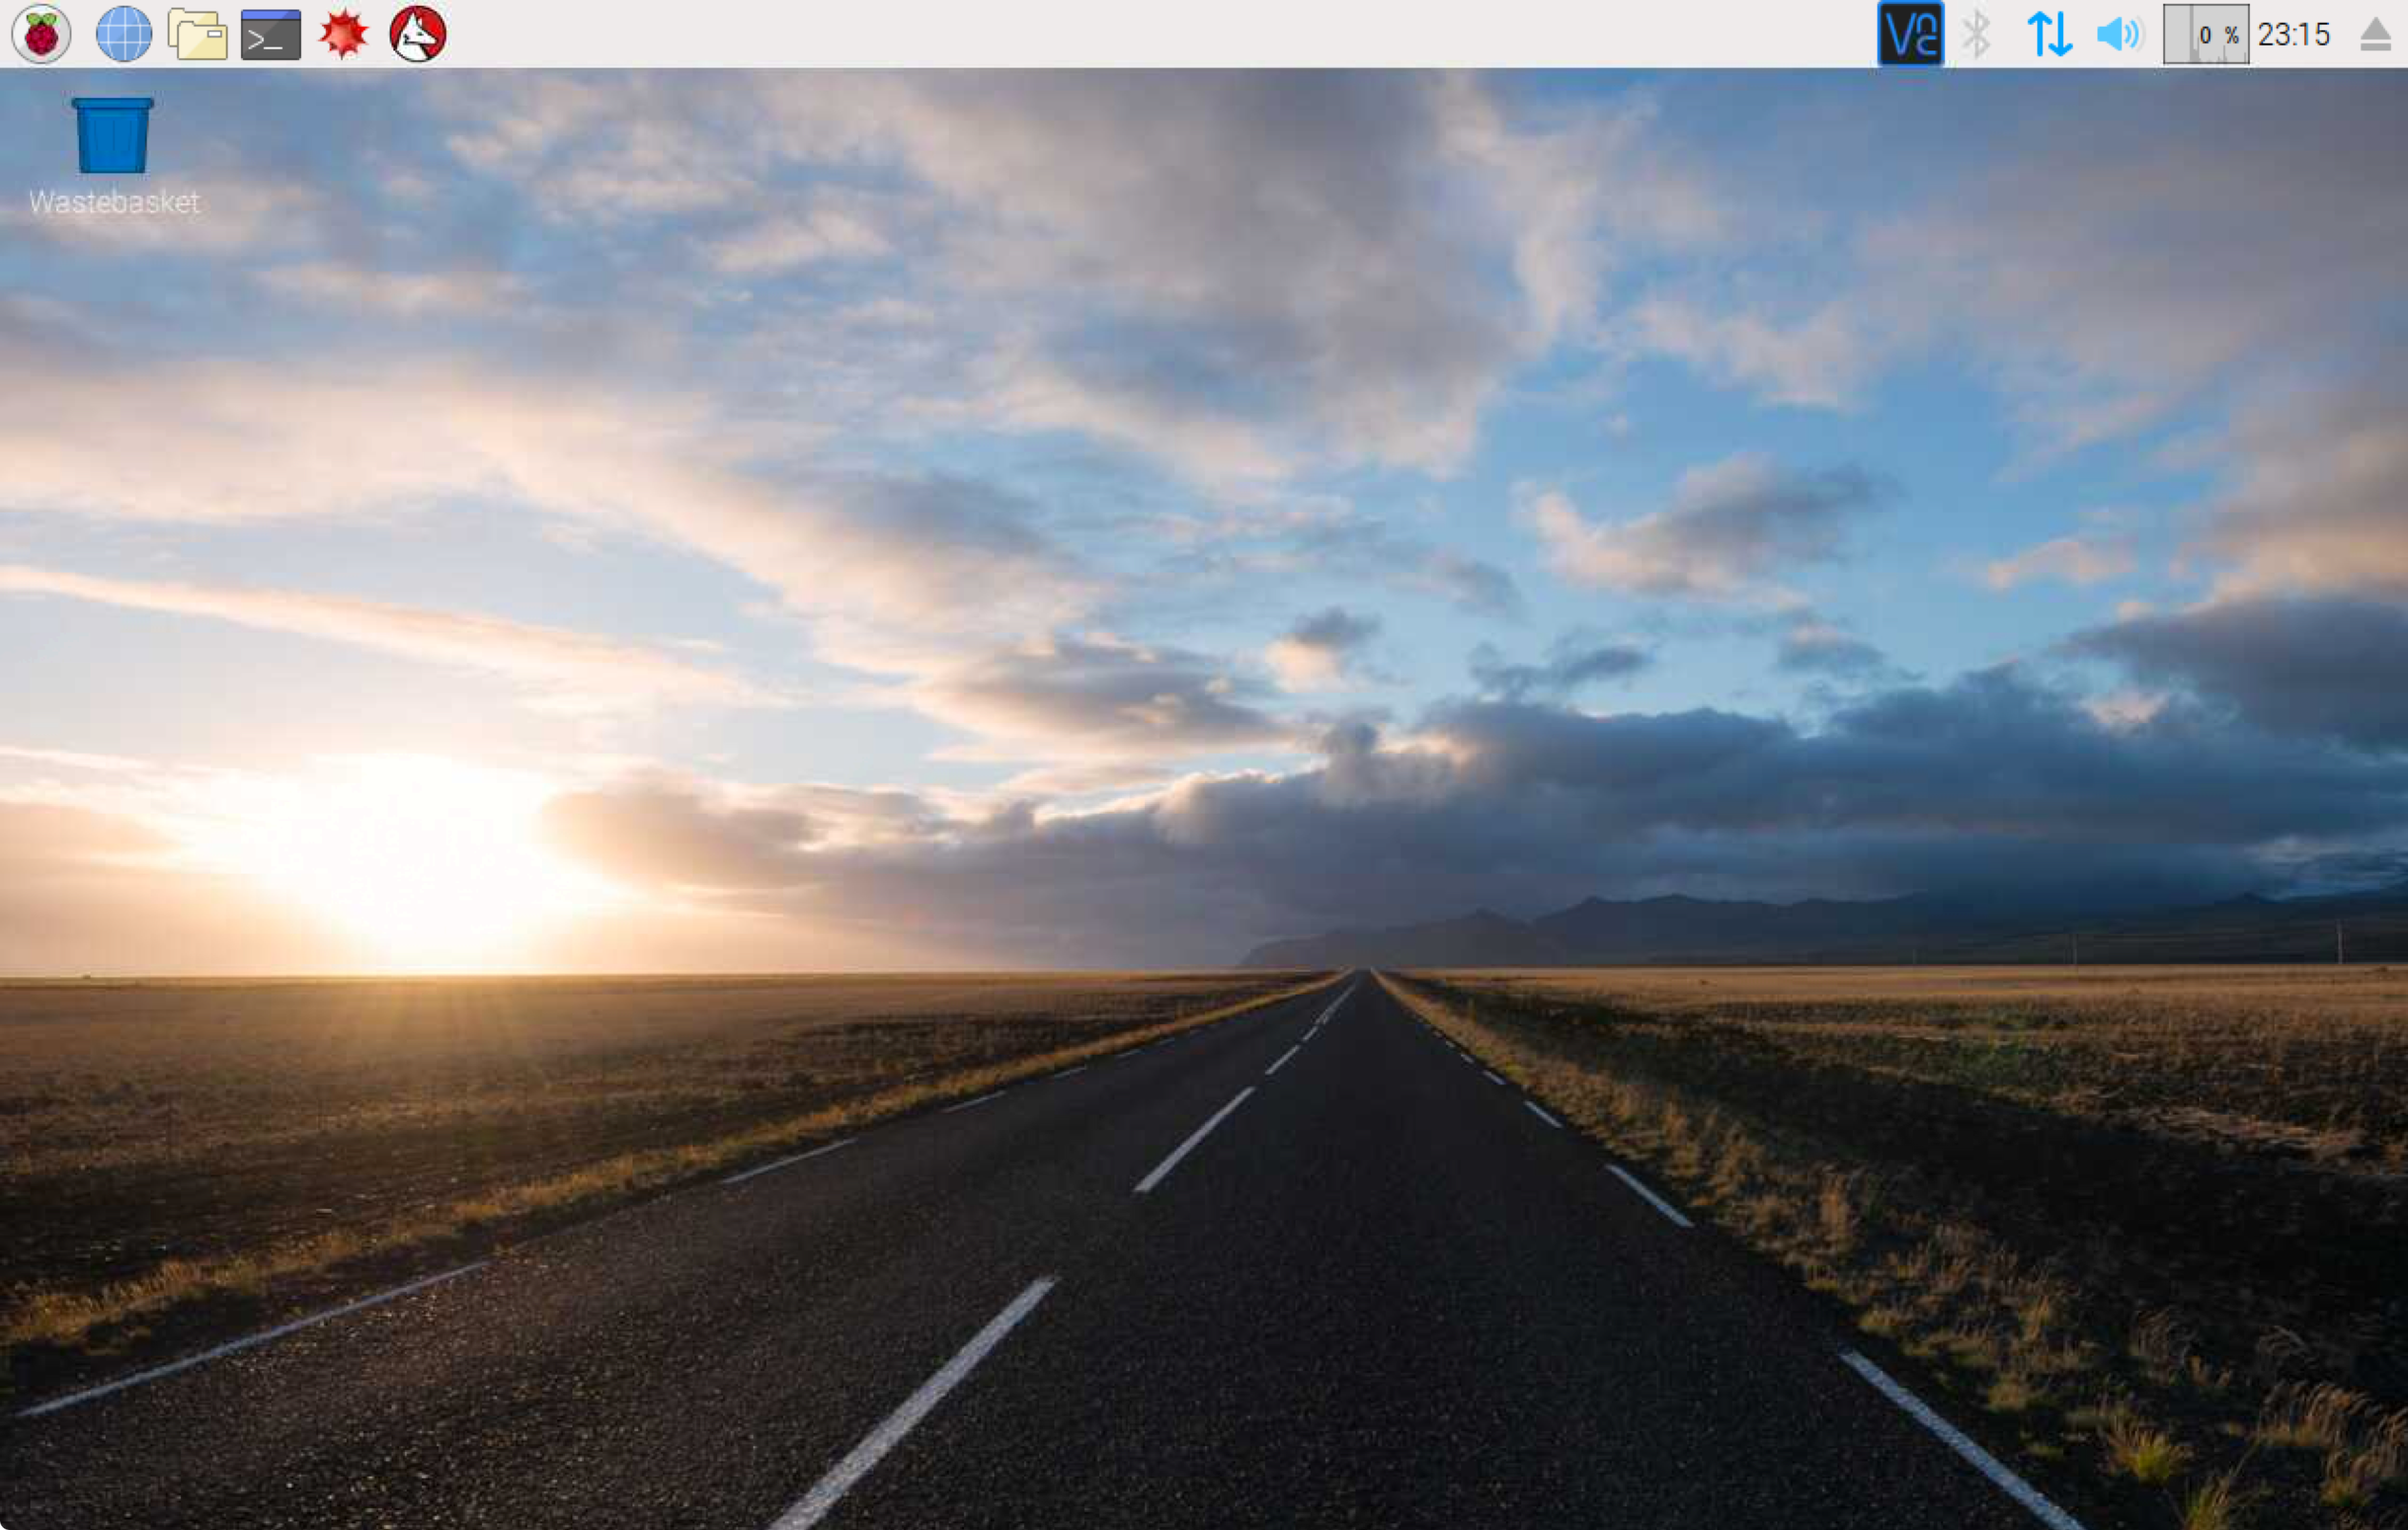
\includegraphics[width=15cm]{raspi.png}
\end{center}
\caption{Interface graphique du Raspberry Pi}
\label{interface}
\end{figure}

\subsection{Connexion directe}

La plus simple est bien sûr de se connecter à un écran via le port HDMI. La connexion est directe, et très fiable. Cependant, on n'a pas toujours un écran libre à disposition, et c'est là que les techniques de connexion suivantes pourront montrer leurs avantages.

\subsection{Connexion SSH (\textit{Secure Shell})}

Il s'agit ici de se connecter au terminal du Raspberry Pi. On n'aura pas accès à l'interface graphique, ce qui complique certaines opérations. Cependant, pour lancer un script ou mettre à jour quelques programmes, c'est un moyen rapide d'accéder au Raspberry Pi.

On se connecte au terminal du Raspberry Pi... par le terminal d'un autre ordinateur! Sur Windows, le programme s'appelle Console, sur macOS simplement Terminal. Une fois le programme ouvert, on trouve d'habitude une simple ligne de texte, et beaucoup d'espace dans lequel écrire des commandes.

Voici celle qui nous permet de nous connecter :

\texttt{ssh nom\_utilisateur@serveur}

Quand on configure le Raspberry Pi, un nom d'utilisateur par défaut est créé, il s'agit simplement de \texttt{pi}. Quant au serveur, ce peut-être une URL (une adresse, comme \texttt{raspberry.serveur.com} par exemple), ou bien une adresse IP (plus compliqué, il existe plusieurs types, mais on retiendra qu'il s'agit d'une suite de chiffres séparés par des points, comme ceci par exemple : \texttt{192.168.1.314}).

Nous vous aiderons à trouver l'adresse du serveur.

Une fois qu'on a l'adresse du serveur, on entre la commande, et un mot de passe est demandé. A nouveau, le Raspberry Pi en a un par défaut : \texttt{raspberry}.

On entre le mot de passe (il ne s'affiche pas, c'est tout-à-fait normal, il faut le taper à l'aveugle), et on a enfin accès au terminal du Raspberry Pi! Pour voir si tout fonctionne, essayez de taper la commande \texttt{uptime}. C'est le temps qu'est resté allumé votre Raspberry Pi depuis qu'on l'a branché à l'alimentation!

\subsection{Connexion VNC}

Ce type de connexion à distance est beaucoup plus agréable : on accède à l'interface graphique, mais via Internet, et non plus via un câble. Ce qui veut dire que si votre appareil est branché à Internet, vous pouvez potentiellement y accéder depuis n'importe où dans le monde!

Pour activer VNC sur le Raspberry Pi, il faut aller dans le terminal, et taper la commande \texttt{sudo raspi-config}. Puis sur l'interface qui s'affiche, on descend avec les flèches du clavier jusqu'à \texttt{Interfacing Options}. On valide avec la touche Entrée. L'option \texttt{VNC} apparaît, il suffit de l'activer.

On va aussi modifier la résolution tant qu'on y est. Il faut cette fois se rendre sur \texttt{Advanced Options} $\rightarrow$ \texttt{Resolution}. Une résolution de 1280x1024 devrait suffire!

\begin{figure}[h!]
\begin{center}
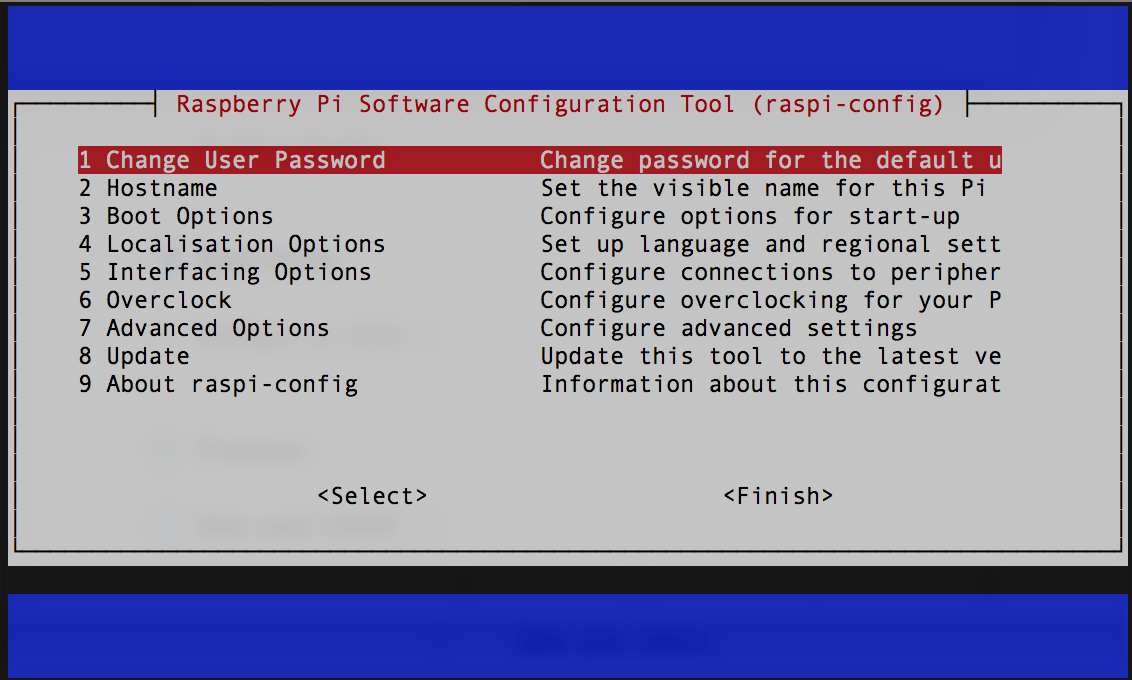
\includegraphics[width=8cm]{raspi-config.png}
\end{center}
\caption{raspi-config}
\label{raspi-config}
\end{figure}

C'est tout pour la configuration sur le Raspberry Pi! A partir de maintenant, plus besoin d'y toucher. Sur notre autre ordinateur maintenant, il faut télécharger un client VNC : \url{https://www.realvnc.com/en/download/vnc/}.

En lançant le programme VNC Connect, il nous est demandé l'adresse du serveur VNC. C'est la même que pour le serveur qu'on a du indiquer lors de la connexion SSH. Ensuite, une fenêtre s'ouvre pour demander l'utilisateur et le mot de passe. Rappelez-vous : par défaut, il s'agit respectivement de \texttt{pi} et \texttt{raspberry}.

%\section{Mettre à jour son Raspberry Pi}
%Raspbian possède une fonction très pratique : on peut mettre à jour tous ses programmes, en même temps et avec seulement deux commandes très pratiques!

Tapez simplement successivement dans le terminal (via SSH ou via l'interface graphique du Raspberry Pi)/

\texttt{sudo apt-get update}

\texttt{sudo apt-get upgrade}

Il est possible qu'une confirmation soit demandée : tapez simplement \texttt{yes} ou \texttt{Y}, selon les cas.
Après quelques téléchargements et installations diverses, c'est fini : tout l'appareil est à jour! Facile, non?

%\section{Installer Python 3}
%Par défaut, le Raspberry Pi n'est plus livré avec Python 3. Heureusement, c'est facile à installer! Tapez successivement les lignes suivantes dans le terminal :\\
%\begin{lstlistings}
%wget https://www.python.org/ftp/python/3.6.0/Python-3.6.0.tgz\\
%tar xzvf Python-3.6.0.tgz\\
%cd Python-3.6.0/\\
%./configure\\
%make\\
%sudo make install\\
%\end{lstlistings}
%
%\section{Mini-jeu}
%Exercice à réaliser en cours.
%
%\section{Capteur d'humidité et de température}
%Dans votre matériel, vous disposez d'un capteur d'humidité et de température. Il est possible de le connecter au Raspberry Pi, et de récupérer les données grâce à... Python!

Il faut d'abord installer le module correspondant. L'installation nécessite quelques commandes à taper dans le terminal :\\
\begin{lstlistings}
sudo apt-get update\\
sudo apt-get install build-essential python-dev\\
wget https://github.com/adafruit/Adafruit\_Python\_DHT/archive/master.zip\\
unzip master.zip\\
cd Adafruit\_Python\_DHT-master/\\
sudo python setup.py install\\
\end{lstlistings}

Ensuite, on peut écrire un script en Python pour lire la température et l'humidité.

\begin{python}
# module du senseur
import Adafruit_DHT

# Pin GPIO
pin = 23

# lit les donnees, et les enregistre dans des variables humidity et temperature
humidity, temperature = Adafruit_DHT.read_retry(sensor, pin)

# affiche les donnees, ou un message d'erreur
if humidity is not None and temperature is not None:
    print('Temperature={0:0.1f}*C  Humidite={1:0.1f}%'.format(temperature, humidity))
else:
    print('Erreur de lecture, reessayez!')
\end{python}

C'est juste un exemple d'utilisation du module, mais avec tout ce qu'on a déjà appris, on va pouvoir faire des choses bien plus intéressantes!
%
\section{Mini-jeu: Snake!}

Pour vous permettre de pratiquer votre talent en programmation, nous vous proposons de créer un petit jeu vidéo, le célèbre Snake.

Vous ne connaissez pas Snake ? Il s'agit d'un jeu vidéo, popularisé par Nokia, qui consiste à guider au clavier un serpent pour lui donner à manger des pommes apparaissant sur le plateau de jeu. Malheureusement pour lui, plus il mange plus il grandit, et il lui est défendu de se mordre lui-même (c-à-d de marcher sur son corps).

Pour cela, nous allons utiliser une bibliothèque logiciel (un module) nommé Pygame, qui permet de développer rapidement des jeux vidéos en Python. Cette bibliothèque permet notamment d'avoir une interface graphique pour votre jeu avec un minimum d'efforts.

Dans le cadre de cette semaine, vous n'aurez pas l'occasion de coder l'ensemble du jeu; c'est bien trop long (et parfois pas très évident). A la place, nous vous proposons de compléter une partie des fonctions utilisées par ce jeu, et de partir du code existant pour l'améliorer et, qui sait, en faire le prochain jeu à succès de la planète :-) !

\section{Utilisation du Raspberry Pi: un radar coloré!}

Maintenant que vous savez utiliser Python ainsi que le Raspberry Pi, nous vous proposons d'utiliser certaines des fonctionnalités du Raspberry qui le rendent populaire.

Avez-vous remarqué la rangée de petits pics métalliques sur le côté de celui-ci ? Il s'agit de connecteurs nommés GPIO (general purpose input/output) qui permettent de connecter toutes sortes de choses au Raspberry Pi: des capteurs, des afficheurs, des DEL \dots.

Nous vous proposons de réaliser un radar détectant les objets s'en approchant en utilisant les différents éléments mis à votre disposition. Attention: suivez bien les instructions données pour éviter d'endommager votre Raspberry.

\chapter{Conclusion}

Durant cette semaine, vous avez appris les bases du Python : variables, conditions, boucles, fonctions, listes, etc. On a donné un introduction à la programmation orienté-objet. Libre à vous désormais de poursuivre cet apprentissage! Le Python est un des langages les plus utilisés, ce qui veut dire qu'il y a aussi énormément de ressources en ligne pour apprendre par soi-même.

On pense notamment à l'excellent OpenClassrooms \footnote{\url{https://openclassrooms.com/courses/apprenez-a-programmer-en-python}}, ou à ce tutoriel sur Développez.com \footnote{\url{https://python.developpez.com/cours/apprendre-python3/}}.\\

Vous avez aussi découvert le Raspberry Pi. Étonnant petit ordinateur, il n'en est pas moins capable! D'autres curieux tels que vous ont utilisé leur Raspberry Pi dans des projets surprenants! Certains sont listés sur Instructables\footnote{\url{http://www.instructables.com/id/Raspberry-Pi-Projects/}}, avec des explications pas-à-pas.\\

Enfin, nous espérons que vous avez apprécié ce stage, et que vous continuerez à explorer les infinies possibilités de l'informatique!


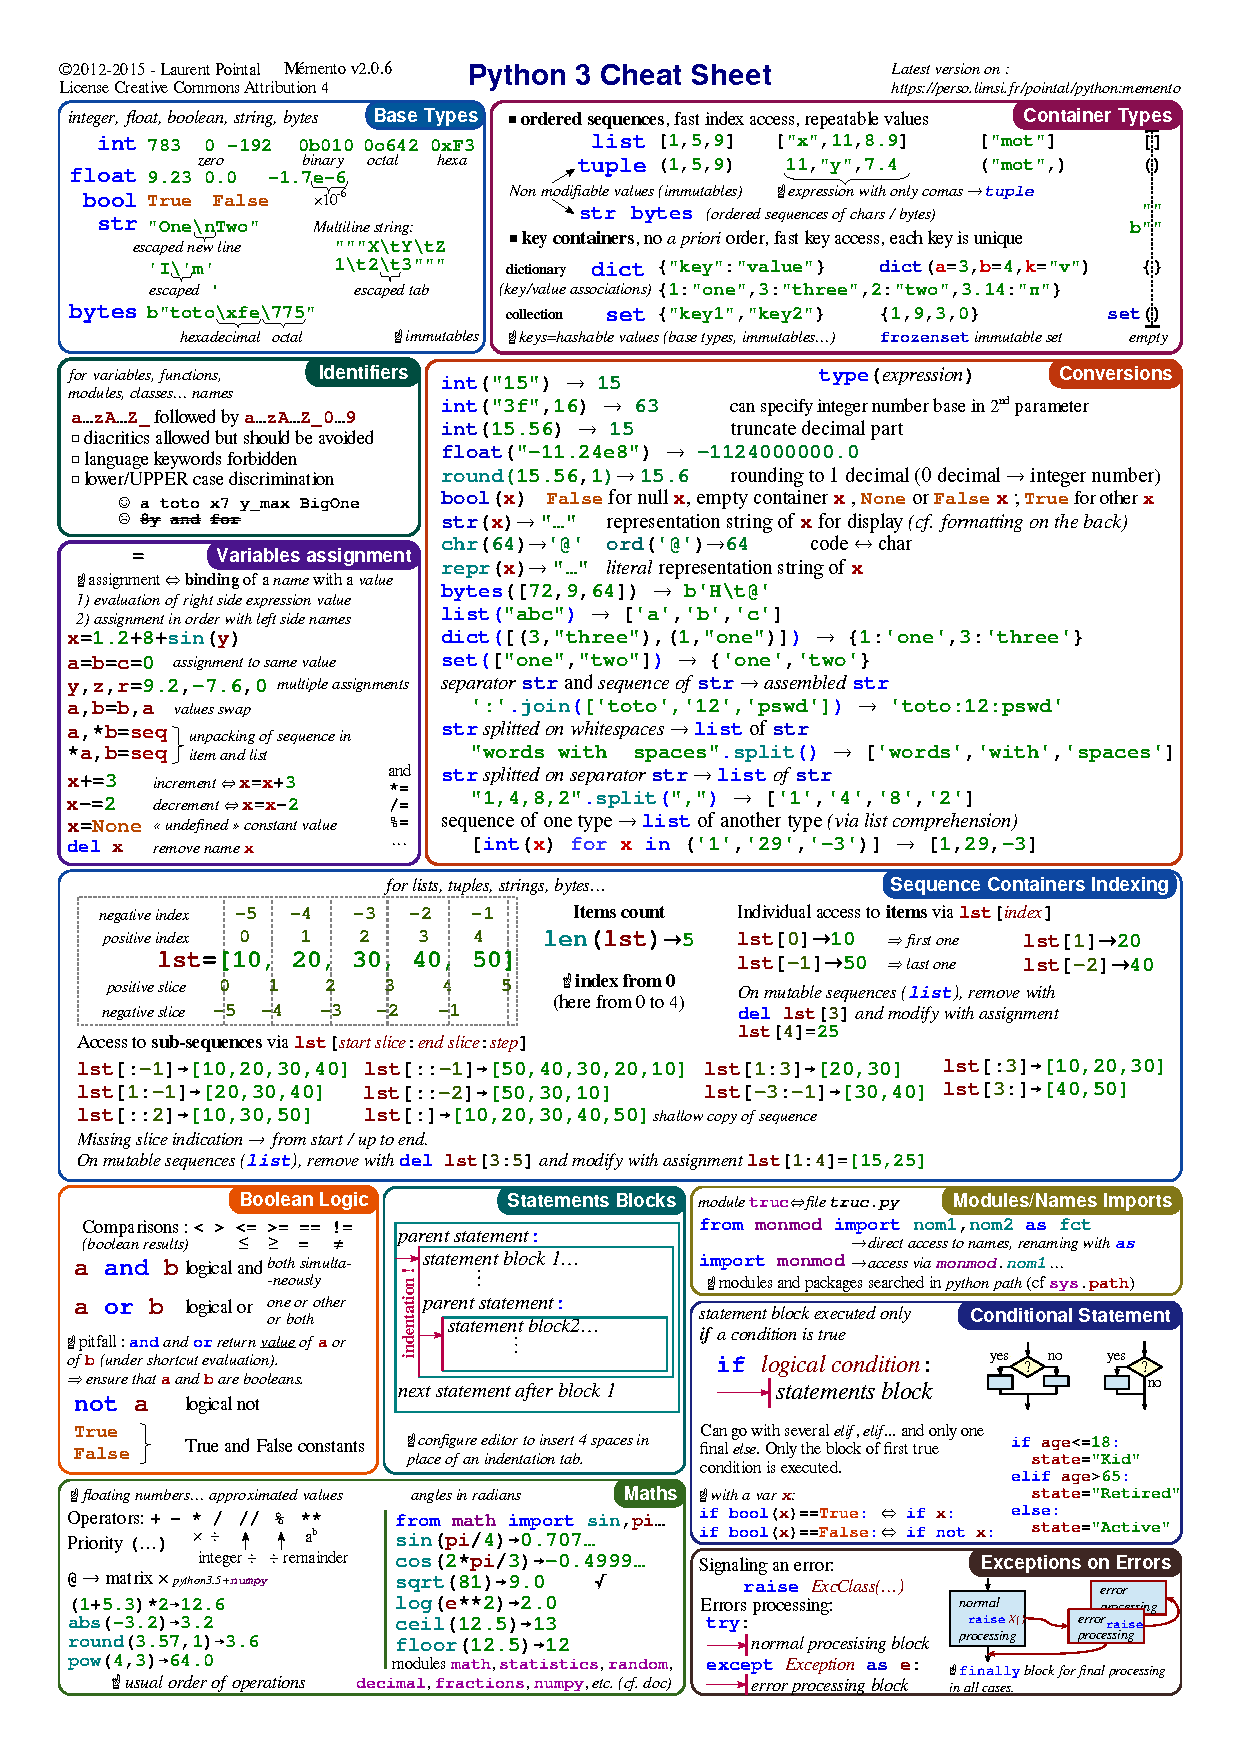
\includepdf[pages={1,2}]{memento.pdf}
\end{document}
